%POLAR COORDINATES
%The print template for A4 paper (portrait)
%Author: Zoran Nikolic
\documentclass[12pt]{article}
\usepackage[margin=0.5in,paper=a4paper]{geometry} %Shrinking margins to 0.5in
\usepackage[x11names]{xcolor}                     %Additional colors
% TikZ graphivc language is described in: http://cremeronline.com/LaTeX/minimaltikz.pdf
\usepackage{tikz}
% For the numeric value calculation look this link: https://tex.stackexchange.com/questions/337831/pgfmathparse-basic-usage 

\begin{document}
\thispagestyle{empty} %Please, no page numbers or similar
{\fontfamily{qhv}\selectfont
  \begin{center}
    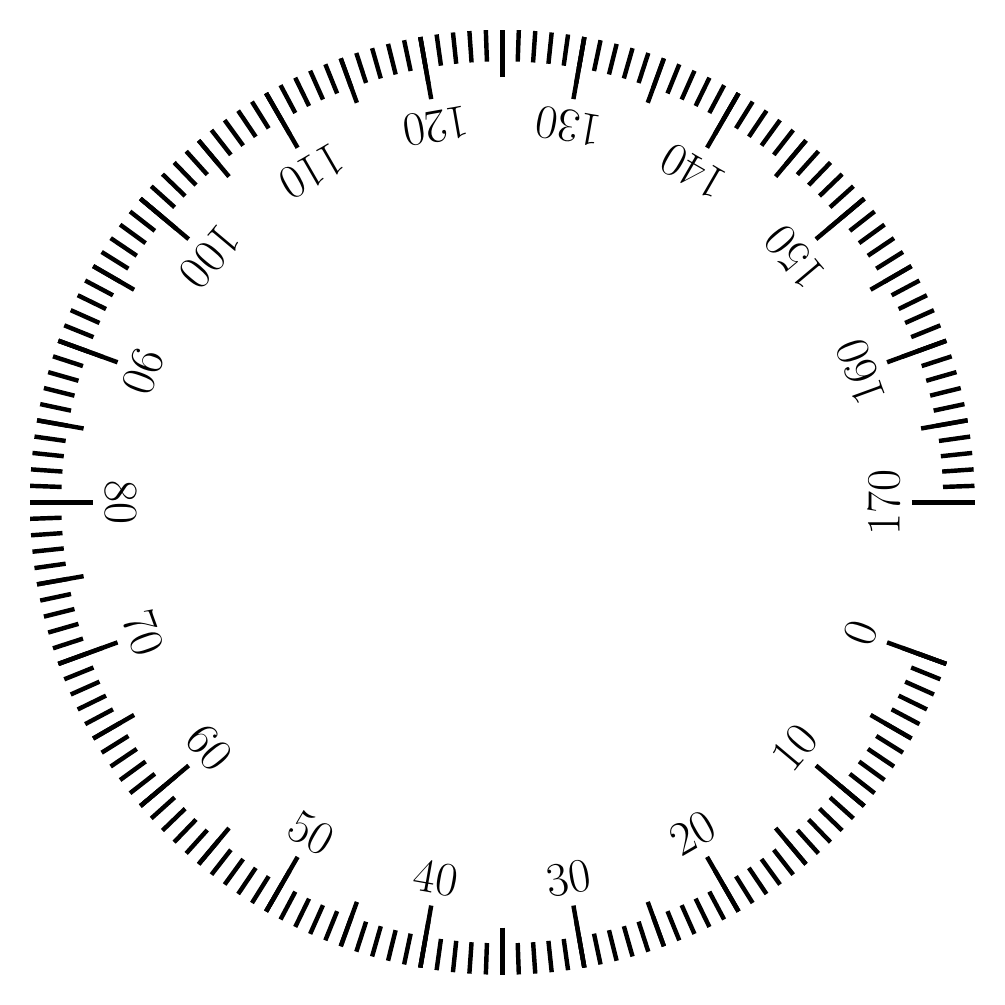
\begin{tikzpicture}
      %1° Rays
      \foreach \a in {0, 2,...,340}
	\draw[ultra thick] (\a:5.6) -- (\a:6);
      %5° Rays
      \foreach \a in {0, 10,...,340}
	\draw[ultra thick] (\a:5.4) -- (\a:6);      
      %10° Rays
      \foreach \a in {0, 20,...,340}
	\draw[ultra thick] (\a:5.2) -- (\a:6); 
      %Angle labels  
      \foreach \a in {0, 20,...,340}
        \pgfmathtruncatemacro\result{170-\a/2}
	\draw (\a: 4.85) node {\LARGE\rotatebox{90}{\rotatebox{\a}{\result}}};
    \end{tikzpicture}
  \end{center}
}
\end{document}
